\section{KeystoneJS}
\label{sec:CMS_ksjs}

KeystoneJS is an open source framework for developing database-driven websites, applications and APIs in Node.js, built on Express and MongoDB.
KeystoneJS provides a strong backbone for a simple content management system. Keystone.js is available for free and sits under the MIT license. In addition, there are sixty four contributors to the open source repository and daily commits.
KeystoneJS runs with two of the most powerful elements of Node.js: Express and MongoDB. Express.js is the most popular web application framework for Node.js and MongoDB is a document based database whose queries are written in JavaScript notation. Learning to use both Express and MongoDB alongside KeystoneJS will allow a user to progress and create web applications in Node.js without KeystoneJS. In addition to using popular frameworks with Node.js, the content management system is also built upon an MVC architecture. Learning this Model-View-Controller Architecture will allow a user to take principles away from KeystoneJS and apply them elsewhere in future applications. \cite{cms_ksjs_rev}

There are some key features of KeystoneJS that stand out as needed features of a CMS. The CMS comes prepared with standard data types such as name, email and password which can be easily incorporated into online forms to speed up validation and database storage. KeystoneJS provides an out-of-the-box Admin User Interface which represents the custom fields and content-types created by the user. A user can easily use this to build a website from the ground up, or use this as a CMS during production. Lastly, KeystoneJS provides natural integration with email. It provides a template email system and incorporates integration with MailChimp, a leading mail service for web applications. \cite{cms_ksjs}



\begin {figure}[h]
\graphicspath{{images/chapter_cms/}}
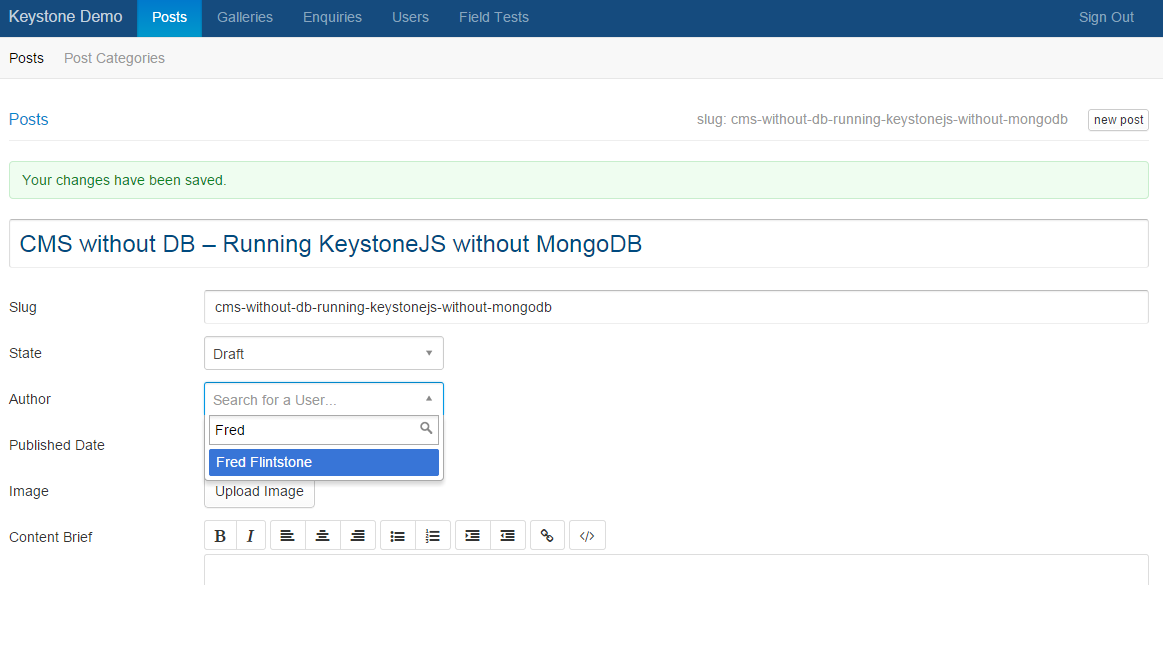
\includegraphics[width=\textwidth]{ksjs_dash}
\caption{KeystoneJS Dashboard}
\end {figure}